\documentclass[aspectratio=1610,11pt]{beamer}
\usepackage[T1]{fontenc}
\usepackage{lmodern,microtype,booktabs,tabularx,array,colortbl,tikz,listings}
\usetikzlibrary{arrows.meta,positioning,calc}
\definecolor{navy}{HTML}{19344B}
\definecolor{teal}{HTML}{087F8C}
\definecolor{muted}{HTML}{607080}
\definecolor{mint}{HTML}{E5F2EE}
\definecolor{paper}{HTML}{F2F5F7}
\definecolor{amber}{HTML}{FFF0D8}
\setbeamercolor{normal text}{fg=navy,bg=white}
\setbeamercolor{frametitle}{fg=navy}
\setbeamercolor{structure}{fg=teal}
\setbeamercolor{block title}{fg=teal,bg=white}
\setbeamercolor{block body}{fg=navy,bg=white}
\setbeamersize{text margin left=8mm,text margin right=8mm}
\setbeamertemplate{navigation symbols}{}
\setbeamertemplate{headline}{}
\setbeamertemplate{frametitle}{\vspace{3mm}\usebeamerfont{frametitle}\insertframetitle\par\vspace{2mm}{\color{teal}\hrule height .5pt}}
\setbeamerfont{frametitle}{size=\large,series=\bfseries}
\setbeamertemplate{footline}{\hspace{8mm}\textcolor{muted}{\tiny DOCQUORUM\quad /\quad REAL-DOCUMENT WALKTHROUGH}\hfill\textcolor{muted}{\tiny\insertframenumber}\hspace{8mm}\vspace{2mm}}
\setlength{\parskip}{4pt}
\newcommand{\tagline}[1]{{\scriptsize\color{teal}\bfseries #1}\par\vspace{1mm}}
\newcommand{\source}[1]{\vfill{\fontsize{5.7}{6.8}\selectfont\color{muted}Source: #1\par}}
\newcommand{\takeaway}[1]{\par\vspace{2mm}\colorbox{mint}{\parbox{\dimexpr\linewidth-2\fboxsep}{\small\strut #1\strut}}}
\newcommand{\lbl}[1]{{\color{teal}\bfseries #1}\par}
\newcommand{\mono}[1]{\texttt{\detokenize{#1}}}
\newcommand{\state}[3]{\colorbox{#1}{\parbox[c][13mm][c]{.27\linewidth}{\centering\scriptsize #2\\[1mm]\large\bfseries #3}}}
\lstset{basicstyle=\ttfamily\scriptsize,columns=fullflexible,keepspaces=true,showstringspaces=false,breaklines=true,backgroundcolor=\color{paper},frame=none,xleftmargin=2mm,xrightmargin=2mm,aboveskip=2mm,belowskip=1mm}
\begin{document}

\begin{frame}[plain]
\centering
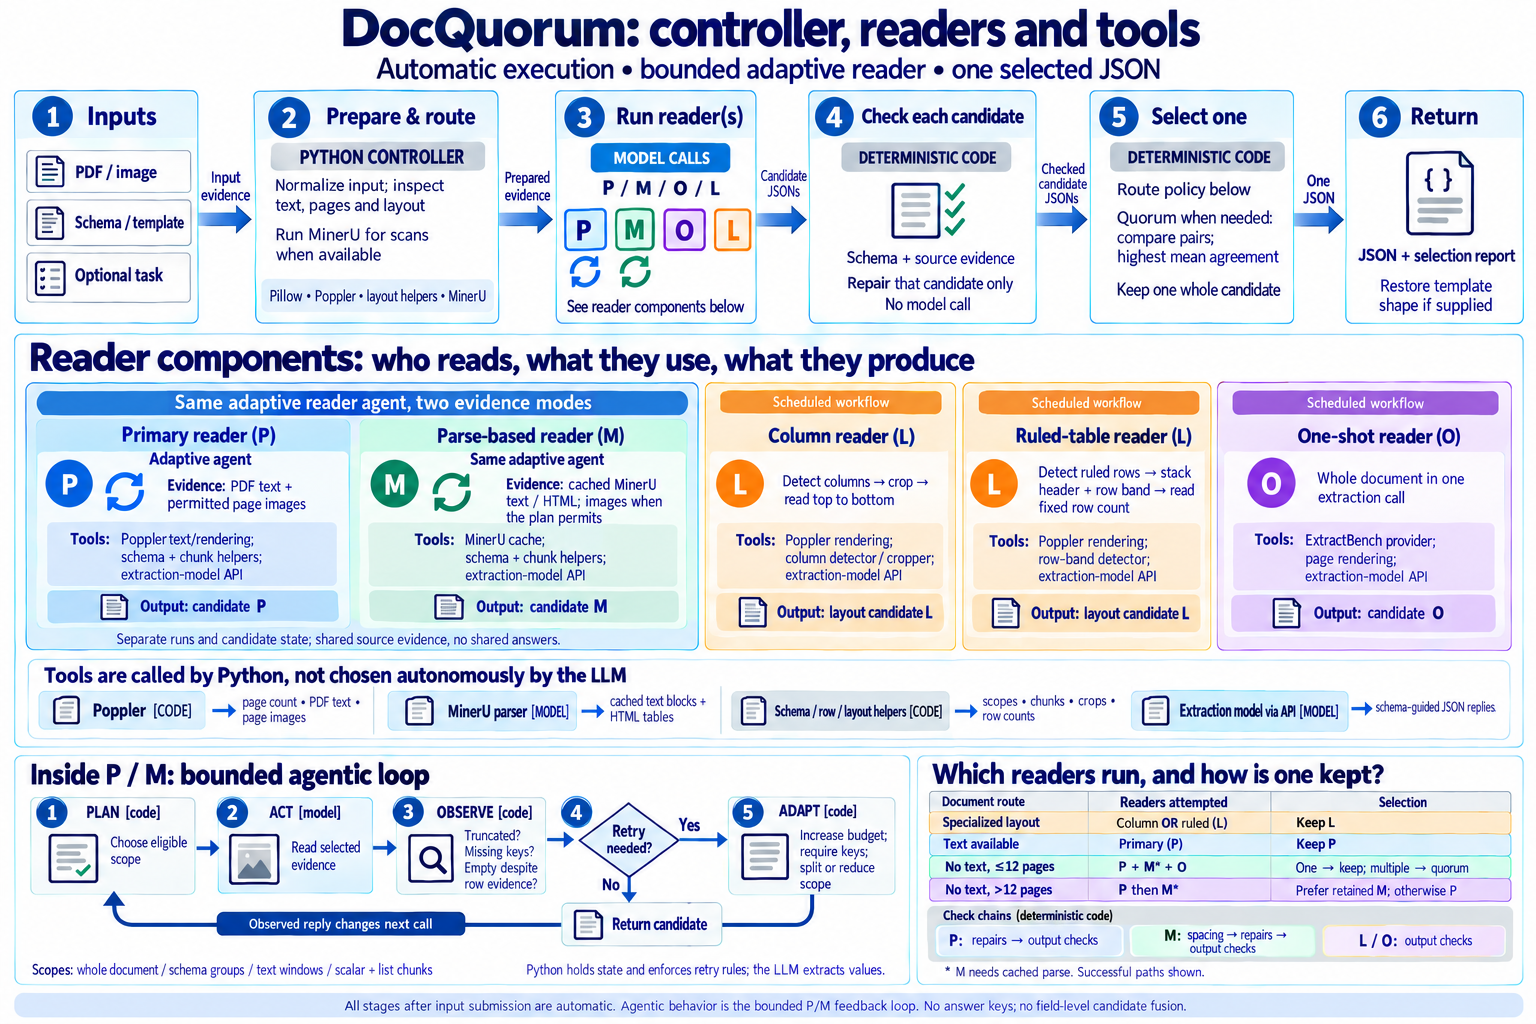
\includegraphics[width=\linewidth,height=.95\textheight,keepaspectratio]{assets/pipeline.png}
\end{frame}

\begin{frame}{1\quad Start with a real document}
\tagline{INPUT / OKLAHOMA COUNTY PURCHASE ORDER}
\begin{columns}[T]
\begin{column}{.34\linewidth}\centering
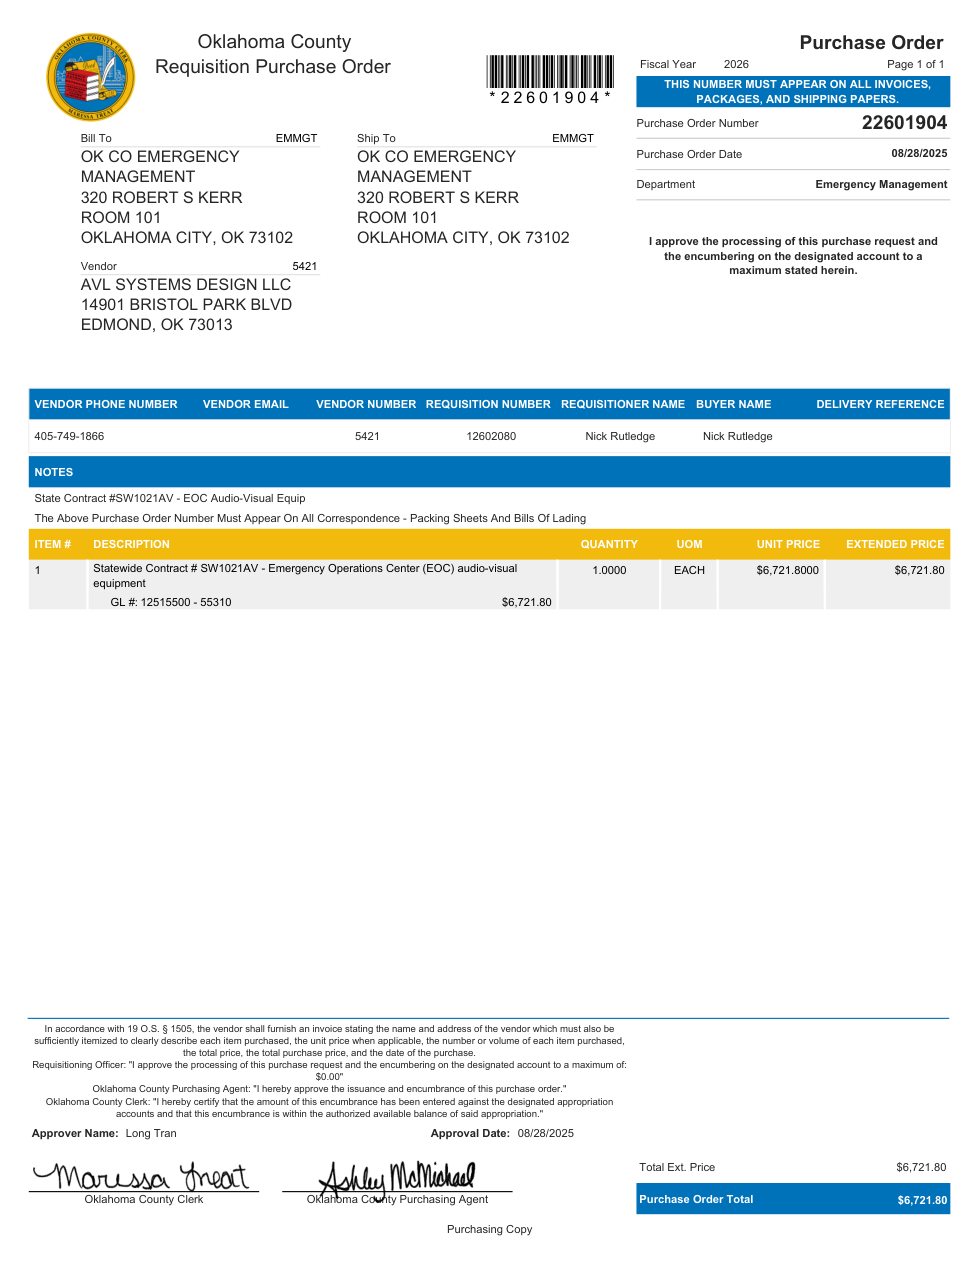
\includegraphics[height=51mm]{assets/po-digital.png}
\end{column}
\begin{column}{.63\linewidth}
\lbl{What the document contains}
\begin{tabular}{@{}ll@{}}
PO number & \textbf{22601904}\\
Date & 28 August 2025\\
Vendor & AVL Systems Design LLC\\
Ordered items & One audiovisual-equipment line\\
Total & \textbf{\$6,721.80}
\end{tabular}\par
\vspace{4mm}
\lbl{What we want back}
A structured object: PO number, vendor, line items, prices and total. The schema tells the reader which fields to extract.
\end{column}
\end{columns}
\takeaway{The document supplies the evidence. The schema defines the answer's structure.}
\source{ExtractBench short / oklahoma\_county\_purchase\_order\_avl\_systems. Original PDF bundled in examples/.}
\end{frame}

\begin{frame}[fragile]{2\quad Tell the reader what to extract}
\tagline{INPUT / SCHEMA OR TEMPLATE + OPTIONAL TASK}
\begin{columns}[T]
\begin{column}{.49\linewidth}
\lbl{Schema: selected actual field types}
\begin{lstlisting}
{
  "type": "object",
  "properties": {
    "po_number": {
      "anyOf": [
        {"type": "string"},
        {"type": "null"}
      ]
    },
    "line_items": {"type": "array"}
  }
}
\end{lstlisting}
\scriptsize The complete schema also describes every field and each line-item property.
\end{column}
\begin{column}{.47\linewidth}
\lbl{Alternative: a template}
\begin{lstlisting}
{
  "po_number": "",
  "line_items": [{
    "description": "",
    "quantity": "",
    "unit_price": ""
  }]
}
\end{lstlisting}
\lbl{Optional task}
\small ``Extract every ordered item. Exclude totals and blank filler rows.''
\end{column}
\end{columns}
\source{Left: excerpt of the real PO schema. Right: teaching template and task, not inputs to the archived benchmark run.}
\end{frame}

\begin{frame}{3\quad First ask: what evidence is available?}
\tagline{PREPARE / THE SAME PO AS A DIGITAL PDF AND A DEGRADED SCAN}
\begin{columns}[T]
\begin{column}{.49\linewidth}
\lbl{Digital PDF: usable embedded text}
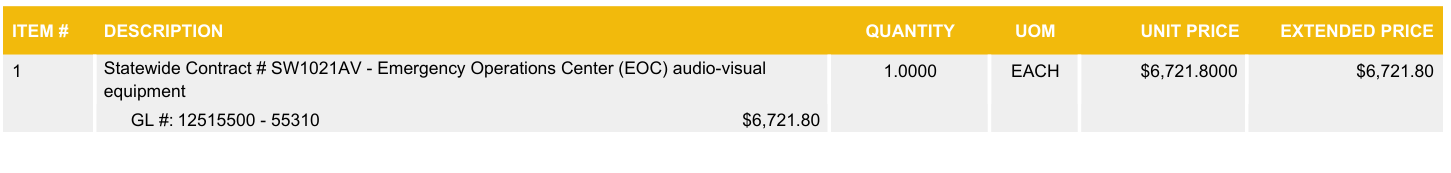
\includegraphics[width=\linewidth]{assets/po-table-digital.png}
\small\textbf{4,995 embedded characters.}\\One primary reading, using text and page images when the plan permits.
\end{column}
\begin{column}{.49\linewidth}
\lbl{Degraded scan: no embedded text}
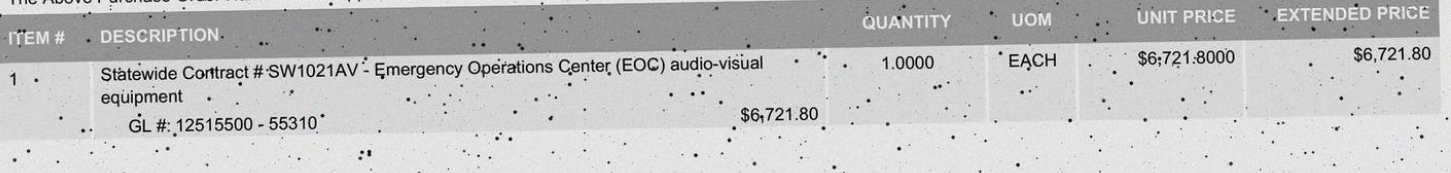
\includegraphics[width=\linewidth]{assets/po-table.png}
\small\textbf{0 embedded characters.}\\At one page: primary, cached-parse and one-shot readings can be compared.
\end{column}
\end{columns}
\vspace{4mm}
\colorbox{paper}{\parbox{\dimexpr\linewidth-2\fboxsep}{\small\textbf{A scan can still contain OCR text.} The real Texas W-14 example contains 931 embedded characters, so it follows the text-available route. Appearance alone does not choose the route.}}
\takeaway{Layout is checked first; otherwise embedded text and page count determine the route.}
\source{Archived front-end measurements from the real digital PO, its benchmark-corrupted derivative, and Texas W-14 form.}
\end{frame}

\begin{frame}[fragile]{4\quad MinerU turns the table into readable evidence}
\tagline{PARSE / ACTUAL TABLE CROP AND CACHED MINERU OUTPUT}
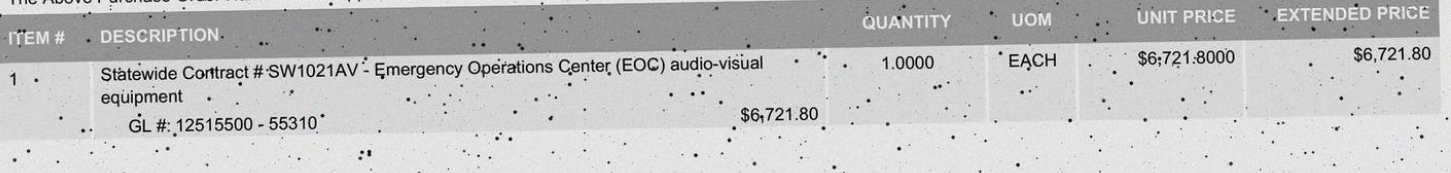
\includegraphics[width=\linewidth,height=18mm,keepaspectratio]{assets/po-table.png}
\begin{columns}[T]
\begin{column}{.58\linewidth}
\lbl{Cached HTML excerpt}
\begin{lstlisting}
<tr><td>1</td>
<td>Statewide Contract # SW1021AV ...</td>
<td>1.0000</td><td>EACH</td>
<td>$6,721.8000</td>
<td>$6,721.80</td></tr>
\end{lstlisting}
\end{column}
\begin{column}{.38\linewidth}
\lbl{Reader maps cells to the schema}
\begin{lstlisting}
"quantity": 1,
"unit_price": 6721.8,
"extended_price": 6721.8
\end{lstlisting}
\end{column}
\end{columns}
\takeaway{The parse is text and HTML, not the final task JSON. The reader still has to interpret it.}
\source{Actual cached MinerU parse for the degraded PO; description shortened with ellipsis. Full unedited parse is bundled.}
\end{frame}

\begin{frame}{5\quad Change the view when layout defines the records}
\tagline{READ / TWO REAL SPECIALIZED ROUTES}
\begin{columns}[T]
\begin{column}{.48\linewidth}
\lbl{Column flow: Oklahoma register}
\begin{minipage}[t]{.42\linewidth}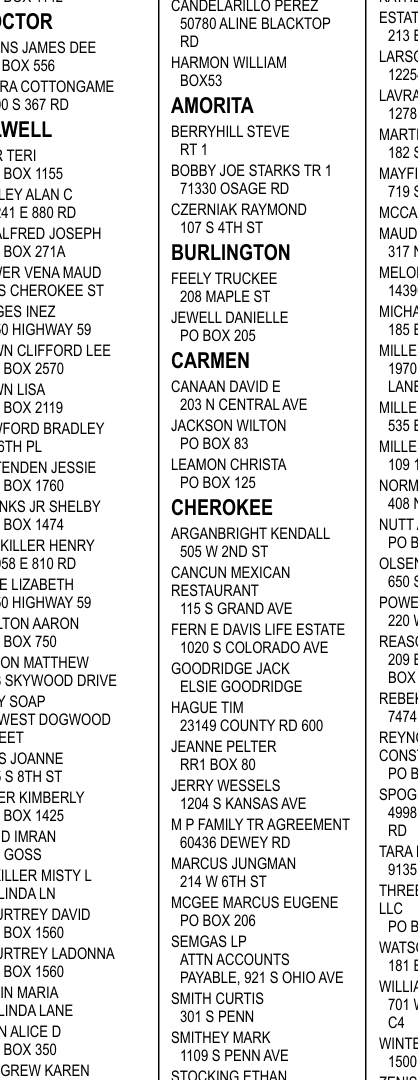
\includegraphics[height=35mm]{assets/columns-detail.png}\end{minipage}\hfill
\begin{minipage}[t]{.54\linewidth}\small Seven columns per page.\par Crop a column. Read top to bottom. Join continuation fragments.\end{minipage}
\end{column}
\begin{column}{.48\linewidth}
\lbl{Ruled table: FTX scanned list}
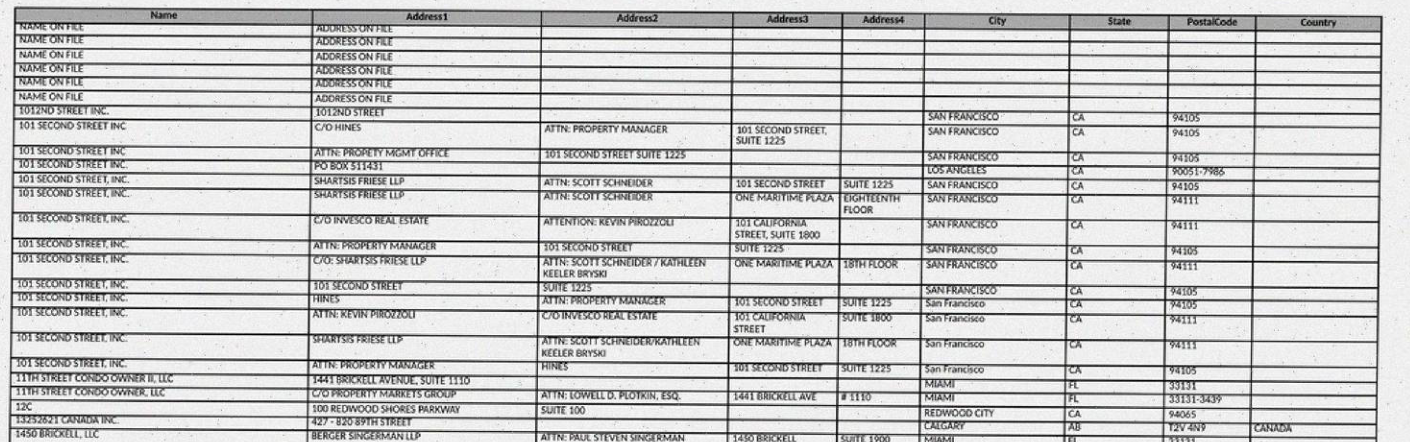
\includegraphics[width=\linewidth,height=25mm,keepaspectratio]{assets/ruled-detail.png}
\small Stack the header above a band of up to 12 rows. Require one output entry per detected row.
\end{column}
\end{columns}
\takeaway{Give the model the region that defines a record: a column or a counted row band.}
\source{Real source-page excerpts: Oklahoma unclaimed-property register, p.2; corrupted FTX creditor list, p.2. Schemas and page PDFs bundled.}
\end{frame}

\begin{frame}[fragile]{6\quad An incomplete reading can trigger another model call}
\tagline{READ / A REAL REQUIRED-FIELD RETRY}

\includegraphics[width=\linewidth]{assets/po-header-fields.png}
\vspace{3mm}
\begin{columns}[T]
\begin{column}{.45\linewidth}
\lbl{First stored reply}
\begin{lstlisting}
"po_number": "22601904"

requisition_number: <absent>
\end{lstlisting}
\end{column}
\begin{column}{.08\linewidth}\vspace{8mm}\Huge\color{teal}$\rightarrow$\end{column}
\begin{column}{.45\linewidth}
\lbl{Required-field re-read}
\begin{lstlisting}
"po_number": "22601904",
"requisition_number": "12602080"
\end{lstlisting}
\end{column}
\end{columns}
\takeaway{The code observes a missing key and requests another model read: a bounded agentic loop.}
\source{Archived digital-PO first reply and second reply; the printed requisition number is shown above.}
\end{frame}

\begin{frame}{7\quad What does a deterministic check actually do?}
\tagline{CHECK / ONE CANDIDATE AT A TIME}
\begin{center}
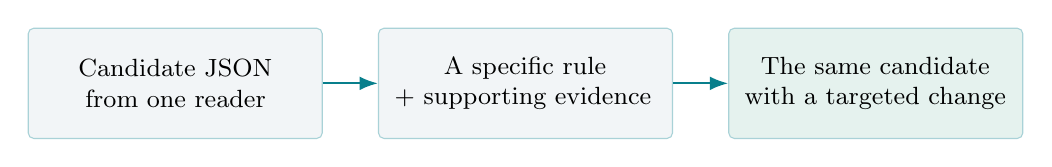
\begin{tikzpicture}[node distance=7mm,box/.style={draw=teal!35,fill=paper,rounded corners=2pt,align=center,text width=35mm,minimum height=14mm,font=\small},arr/.style={-{Latex},thick,teal}]
\node[box] (a) {Candidate JSON\\from one reader};
\node[box,right=of a] (b) {A specific rule\\+ supporting evidence};
\node[box,right=of b,fill=mint] (c) {The same candidate\\with a targeted change};
\draw[arr] (a)--(b);\draw[arr] (b)--(c);
\end{tikzpicture}
\end{center}
\vspace{3mm}
\begin{tabularx}{\linewidth}{@{}p{31mm}XX@{}}\toprule
Example & What authorizes the change? & What changes?\\\midrule
Blank checkbox & Explicit schema convention & \mono{null} becomes \mono{false}\\[2pt]
Rounded number & A uniquely supported printed value & Restore printed precision\\[2pt]
Copied record & Matching values across two arrays & Remove the extra copy\\\bottomrule
\end{tabularx}
\takeaway{A check applies only when its conditions match. It does not certify the whole answer.}
\source{Current docquorum/checks implementation. These three rules are demonstrated with real inputs on the next pages.}
\end{frame}

\begin{frame}[fragile]{8\quad Check example: blank means false, not unknown}
\tagline{SCHEMA-DRIVEN / TEXAS P-4 FORM, ITEM 13}
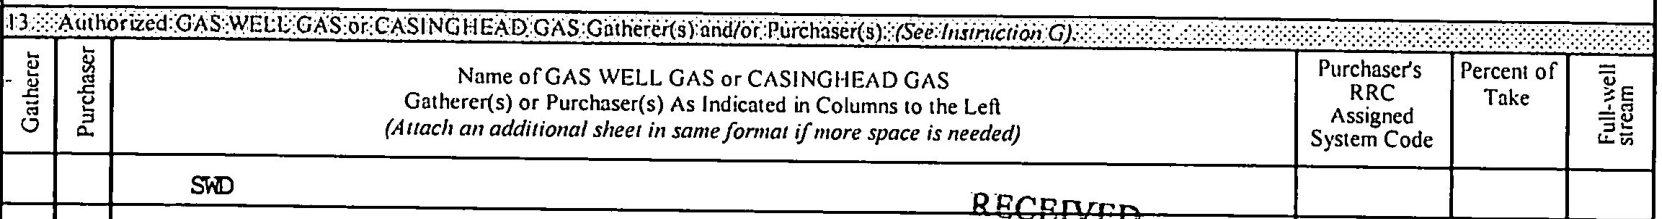
\includegraphics[width=.8\linewidth]{assets/check-checkbox-evidence.png}\par
\small The ``Gatherer'' cell for \textbf{SWD} is blank. The schema explicitly says:\par
\colorbox{paper}{\parbox{\dimexpr\linewidth-2\fboxsep}{\small ``True if the Gatherer checkbox on this row is marked, false if it is blank.''}}
\vspace{1mm}
\begin{center}
\state{amber}{MODEL CANDIDATE}{\texttt{gatherer: null}}\hspace{3mm}{\Large\color{teal}$\rightarrow$}\hspace{3mm}\state{mint}{AFTER THE CHECK}{\texttt{gatherer: false}}
\end{center}
\small\textbf{Why this rule applies:} the field is boolean, its description defines blank as false, and it gives no separate meaning to null.
\takeaway{The check uses the schema convention. It does not look at the image or re-run OCR.}
\source{Real P4-83-211\_35 PDF and stored prediction. Current blank\_boxes.apply replayed without model calls; complete artifacts bundled.}
\end{frame}

\begin{frame}{9\quad Check example: keep the precision printed in the table}
\tagline{TEXT-GROUNDED / BYLINE BANCORP, Q2 2023}
\begin{columns}[T]
\begin{column}{.52\linewidth}
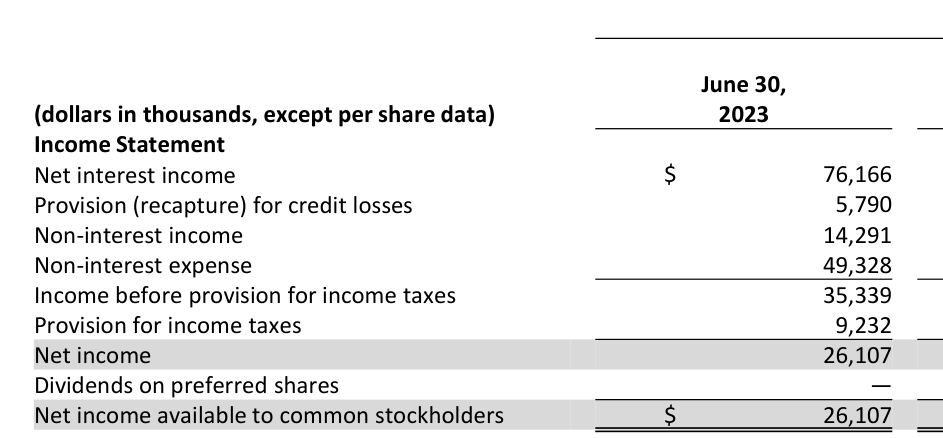
\includegraphics[width=\linewidth]{assets/check-number-evidence.png}
\scriptsize Original table: \textbf{dollars in thousands}. Net income: \textbf{26,107}.
\end{column}
\begin{column}{.44\linewidth}
\lbl{The schema requests millions}
\small The candidate says \textbf{26.11}. That is a rounded version of the source value.\par
Printed 26,107 thousand = \textbf{26.107 million}.
\vspace{2mm}
\colorbox{amber}{\parbox{.88\linewidth}{\small Before\quad\texttt{net\_income: 26.11}}}\par
\colorbox{mint}{\parbox{.88\linewidth}{\small After\quad\texttt{net\_income: 26.107}}}
\end{column}
\end{columns}
\takeaway{The rule restores a uniquely supported printed value; it does not estimate a new number.}
\source{Byline Bancorp investor deck, physical p.18; actual stored candidate. printed\_numbers.apply replay with text extracted from the source PDF.}
\end{frame}

\begin{frame}[fragile]{10\quad Check example: one check was put into two lists}
\tagline{STRUCTURE / PUEBLO SCHOOL DISTRICT CHECK REGISTER}
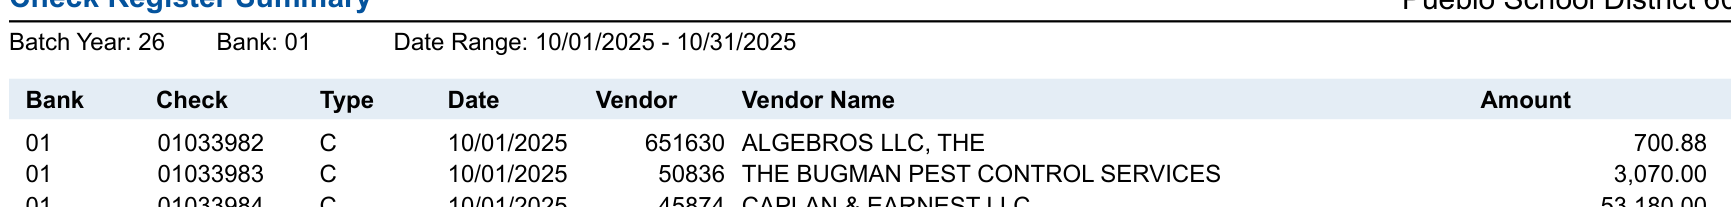
\includegraphics[width=\linewidth]{assets/check-pueblo-evidence.png}
\scriptsize The printed row labels \textbf{01033982 as a check number}, with amount \textbf{700.88}.
\begin{columns}[T]
\begin{column}{.48\linewidth}
\lbl{Keep the actual check}
\begin{lstlisting}
checks[]:
  check_number: "01033982"
  amount: "700.88"
\end{lstlisting}
\end{column}
\begin{column}{.48\linewidth}
\lbl{Remove its copy from batches}
\begin{lstlisting}
batches[]:
  batch_number: "01033982"
  amount: "700.88"
\end{lstlisting}
\end{column}
\end{columns}
\small\textbf{Why it applies:} distinctive values match under different keys. At least three rows, and at least half of the judged batch rows, repeat this pattern.
\takeaway{562 batch entries become 51. All 511 check records stay unchanged.}
\source{Real Pueblo register and stored prediction. copied\_rows.apply replayed; the rule compares arrays, not the page image.}
\end{frame}

\begin{frame}{11\quad Checks do not combine the different readings}
\tagline{CANDIDATES / BACK TO THE DEGRADED PURCHASE ORDER}
\begin{tabularx}{\linewidth}{@{}p{35mm}*{3}{>{\raggedright\arraybackslash}X}@{}}\toprule
Selected field & \textbf{Primary} & \textbf{Parse-based} & \textbf{One-shot}\\\midrule
Requisition number & 12602080 & \texttt{null} & 12602080\\[3pt]
Address excerpt & BRISTOL PARK BLVD & BRISTOL PARK BLVD. & BRISTOL PARK BLVD.\\[3pt]
Description excerpt & GL \#: 12515500 & GL \#: 12515500 & GL \#,12515500\\\bottomrule
\end{tabularx}\par
\vspace{4mm}
\small These are excerpts from \textbf{actual checked candidates}. Each reader used the source independently.
\par The parse candidate omitted the requisition key. The shape check added \texttt{null}; it did not recover the printed number.
\takeaway{Deterministic changes can improve consistency without fixing every missing or incorrect value.}
\source{Archived checked outputs for oklahoma\_county\_purchase\_order\_avl\_systems\_corrupted. Full candidate JSONs are bundled.}
\end{frame}

\begin{frame}[fragile]{12\quad Quorum keeps one complete candidate}
\tagline{SELECT + RETURN / THE STORED PURCHASE-ORDER DECISION}
\begin{columns}[T]
\begin{column}{.45\linewidth}
\lbl{Mean agreement with the others}
\begin{tabular}{@{}lr@{}}\toprule
Primary & 0.9348\\[2pt]
Parse-based & 0.9348\\[2pt]
\rowcolor{mint}\textbf{One-shot: selected} & \textbf{0.9565}\\\bottomrule
\end{tabular}\par
\vspace{3mm}
\small Compare all candidate pairs. Select the highest mean agreement. Ties follow reader order.
\end{column}
\begin{column}{.5\linewidth}
\lbl{Returned JSON: excerpt of one-shot}
\begin{lstlisting}
{
  "po_number": "22601904",
  "requisition_number": "12602080",
  "total_amount": 6721.8,
  "currency": "USD"
}
\end{lstlisting}
\small No fields are borrowed from the other candidates.
\end{column}
\end{columns}
\takeaway{Agreement is not accuracy: in this real example, primary scored better against the answer key.}
\source{Archived agreement.json and final.json. Selection sees candidates and schema, not the answer key. No new model inference.}
\end{frame}

\begin{frame}{Results\quad ExtractBench}
\tagline{95.43 OVERALL / 3RD IN THE PINNED SNAPSHOT}
{\fontsize{5.5}{6.4}\selectfont\setlength{\tabcolsep}{1.5pt}\renewcommand{\arraystretch}{1.07}
\begin{columns}[T]
\begin{column}{.495\linewidth}
\begin{tabularx}{\linewidth}{@{}rXrrrr@{}}\toprule
\# & System & Short & Med. & Long & Overall\\\midrule
1 & LlamaExtract Agentic Plus & 96.94 & 94.45 & 90.18 & 95.91 \\
1 & Pulse (Effort) & 96.46 & 95.01 & 93.51 & 95.91 \\
\rowcolor{mint} 3 & DocQuorum (ours) & 96.34 & 94.11 & 90.41 & 95.43 \\
4 & LlamaExtract Agentic & 96.04 & 92.11 & 91.83 & 94.77 \\
5 & Codex (GPT-6 Sol Evidence) & 95.99 & 92.42 & 87.25 & 94.57 \\
6 & Codex (GPT-5.6 Sol Evidence) & 96.04 & 90.19 & 82.73 & 93.77 \\
7 & Codex (GPT-5.5) & 95.68 & 91.15 & 78.88 & 93.57 \\
8 & Codex (GPT-5.5 Evidence) & 95.59 & 88.72 & 87.97 & 93.35 \\
9 & Pulse (Non-effort) & 93.17 & 92.22 & 89.07 & 92.70 \\
10 & LlamaExtract Cost-Effective & 94.03 & 89.51 & 83.73 & 92.27 \\
11 & Codex (GPT-5.6 Terra Evidence) & 95.60 & 86.69 & 77.36 & 92.26 \\
12 & OpenAI GPT-6 Astra & 97.22 & 90.56 & 31.70 & 91.91 \\
13 & Codex (GPT-5.6 Luna Evidence) & 93.50 & 87.43 & 80.05 & 91.16 \\
14 & Codex (GPT-6 Luna Evidence) & 93.09 & 87.71 & 80.88 & 91.01 \\
15 & Reducto Deep Extract & 94.20 & 80.47 & 92.01 & 90.44 \\
16 & Qwen3.8 Flash Next & 94.82 & 87.81 & 37.74 & 89.88 \\
17 & Qwen3.8 27B & 94.68 & 87.54 & 38.45 & 89.75 \\
18 & Extend (Max Context) & 92.32 & 78.75 & 90.46 & 88.62 \\
19 & Qwen3.6 35B & 92.86 & 86.37 & 36.90 & 88.11 \\
20 & Qwen3.5 35B & 93.52 & 85.27 & 31.73 & 88.00 \\
21 & DeepSeek V4.1 Flash & 94.44 & 81.49 & 22.23 & 87.11 \\
22 & Claude Code (Opus 4.8) & 90.08 & 79.21 & 88.07 & 87.09 \\
23 & Claude Code (Opus 4.8 Evidence) & 90.54 & 79.17 & 77.94 & 86.84 \\
24 & Qwen3.5 9B & 92.31 & 81.12 & 32.22 & 86.10 \\

\bottomrule\end{tabularx}
\end{column}
\begin{column}{.495\linewidth}
\begin{tabularx}{\linewidth}{@{}rXrrrr@{}}\toprule
\# & System & Short & Med. & Long & Overall\\\midrule
25 & Claude Code (Opus 5.5 Evidence) & 89.63 & 77.96 & 80.83 & 86.06 \\
26 & Extend Extract & 89.39 & 84.14 & 47.21 & 85.72 \\
27 & Datalab (Accurate + Balanced) & 89.40 & 85.08 & 42.04 & 85.70 \\
28 & Reducto Extract & 92.97 & 69.59 & 30.65 & 83.41 \\
29 & Kimi K3 & 94.64 & 69.64 & 4.99 & 83.17 \\
30 & Qwen3.5 4B & 89.06 & 76.64 & 27.31 & 82.43 \\
31 & NuExtract3 & 86.41 & 77.01 & 32.71 & 81.02 \\
32 & GLM-5.3 Flash & 96.30 & 51.56 & 27.83 & 80.75 \\
33 & Google Gemini 3.8 Flash & 88.14 & 72.23 & 28.70 & 80.71 \\
34 & Google Gemini 3.5 Flash & 87.87 & 69.76 & 27.90 & 79.84 \\
35 & Lift Datalab 9B & 87.64 & 65.69 & 24.78 & 78.43 \\
36 & OpenAI GPT-5.4 Nano & 77.43 & 76.37 & 35.81 & 74.90 \\
37 & Gemma4 26B & 77.70 & 59.61 & 28.88 & 70.27 \\
38 & Gemma4 E4B & 81.10 & 48.93 & 26.82 & 69.64 \\
39 & InternVL3.5 14B & 80.70 & 39.04 & 19.41 & 66.35 \\
40 & InternVL3.5 8B & 79.26 & 36.62 & 17.57 & 64.63 \\
41 & Qwen3.5 2B & 71.22 & 50.93 & 25.93 & 63.40 \\
42 & Kimi-VL A3B & 69.86 & 34.61 & 18.94 & 57.77 \\
43 & Gemma4 E2B & 63.71 & 28.96 & 14.58 & 51.85 \\
44 & NuExtract 2.0 8B & 62.92 & 23.50 & 6.39 & 49.42 \\
45 & Qwen3.5 0.8B & 57.44 & 26.98 & 6.65 & 46.63 \\
46 & MiniCPM-V 4.5 & 57.39 & 25.30 & 1.13 & 45.85 \\
47 & Gemma4 12B & 53.62 & 30.82 & 13.16 & 45.39 \\
48 & GLM-4.6V Flash & 47.28 & 44.52 & 22.17 & 45.19 \\

\bottomrule\end{tabularx}
\end{column}
\end{columns}}
\vspace{1mm}\scriptsize 370 PDFs; value F1 (\%). All 47 published systems + DocQuorum. Equal scores share a rank.
\source{Maintained docs/results snapshot, 2 Oct 2026; scorer c8e5969. Stored outputs, not fresh inference. ExtractBench was used in development.}
\end{frame}

\begin{frame}{Results\quad UNIKIE-BENCH}
\tagline{82.62 MACRO F1 / 1ST}
\begin{columns}[T]
\begin{column}{.60\linewidth}
{\scriptsize\renewcommand{\arraystretch}{1.03}
\begin{tabularx}{\linewidth}{@{}rXr@{}}\toprule
\# & System & Macro F1\\\midrule
\rowcolor{mint} 1 & DocQuorum (ours) & 82.62 \\
2 & Gemini-3-Pro & 82.37 \\
3 & Qwen3-VL-Plus & 80.20 \\
4 & Qwen3-VL-8B & 79.12 \\
5 & Qwen-VL-Max & 77.77 \\
6 & GLM-4.1V-9B & 69.91 \\
7 & GPT-4o & 69.15 \\
8 & MiMo-VL-7B-RL & 68.88 \\
9 & InternVL3.5-8B & 67.70 \\
10 & GPT-5 & 67.59 \\
11 & MiniCPM-V4.5-8B & 67.15 \\
12 & Claude-Sonnet-4.5 & 66.39 \\
13 & Kimi-VL-A3B & 66.14 \\
14 & Gemma-3-12B & 48.09 \\
15 & Ministral-3-8B & 37.62 \\
16 & SmolVLM2-2.2B & 23.69 \\

\bottomrule\end{tabularx}}
\end{column}
\begin{column}{.34\linewidth}
\vspace{4mm}\lbl{4,472 images}
11 document scenarios.\par\vspace{2mm}
\lbl{Six-reading quorum}
A separate benchmark protocol, including extra-model readings.\par\vspace{2mm}
\small This score is not attributed to the single-document API alone.
\end{column}
\end{columns}
\source{Maintained docs/results snapshot: UNIKIE-BENCH Table 4 and stored DocQuorum evaluation. All 15 published systems + DocQuorum.}
\end{frame}
\end{document}
